% !TeX root = ../praktikum.tex
% !TeX encoding = UTF-8
% !Tex spellcheck = de_DE

Die geometrische Optik ist der Teilbereich der Optik, wo Lichtwellen durch idealisierte Strahlen angenähert werden um den Weg des Lichtes zu (re)konstruieren. Sämtliche Schlussfolgerungen basieren auf diesen vier Axiomen:

\begin{enumerate}
	\item{Axiom:} In homogenem Material verlaufen Lichtstrahlen gerade.
	\item{Axiom:} An der Grenze zwischen zwei homogenen und isotropen Materialien wird das Licht nach dem Reflexionsgesetz reflektiert und nach dem Brechungsgesetz gebrochen.
	\item{Axiom:} Zeit- bzw. Strahlenumkehr, die Richtung eines Lichtstrahles ist belanglos.
	\item{Axiom:} Die Lichtstrahlen beeinflussen sich nicht gegenseitig.
\end{enumerate}

Durch die spezielle Geometrische Form von Sammellinsen ergibt sich ein Brechungswinkel in Abhängigkeit vom Abstand zum Mittelpunkt, der effektiv Strahlen bündeln oder kollimieren kann. Die Brennweite gibt den Abstand an, in dem sich eine punktförmige Lichtquelle befinden muss, um von der Linse kollimiert zu werden. Gleichzeitig ist sie auch die Entfernung in der ein kollimierter Strahl hinter einer Linse gebündelt wird (siehe auch drittes Axiom).

Neben den Effekten der geometrischen Optik gibt es noch Effekte, die sich nicht durch dieses einfache Modell beschreiben lassen. Hierzu zählt die Streuung. Diese kann nach dem Huygenssches Prinzip\cite{_huygenssches_????} beschrieben und mittels der Beschreibung durch die Frauenhoferbeugung\cite{_beugungsintegral_2015} vereinfacht werden. Die wesentliche Erkenntnis hieraus ist, dass ein Lichtstrahl der durch ein Objekt mit einem oder mehreren Spalten, deren Öffnungsbreite in der Größenordnung der Wellenlänge liegt, läuft gestreut, das heißt aufgeweitet, wird. Dieser Strahl wird anschließend auf Grund von Laufzeitunterschieden mit sich selber interferieren. Dabei ist das auf einem, in einem zur Spaltweite großem Abstand befindlichen, Schirm entstehende Muster von der Spaltweite und -anzahl abhängig. Dabei gilt: Je feiner das Spaltmuster, desto größer ist der Abstand zwischen den Interferenzmaxima.

Effektiv wird das Licht also in Teilstrahlen aufgeteilt, deren Winkel abhängig von der Amplitudenstruktur des Objektes ist. Je weiter man sich nun von dem Objekt entfernt, desto größer wird das Verhältnis zwischen Winkel- und räumlichen Informationen. In der Unendlichkeit gibt der Ort eines Maximums nur noch Informationen über die Größenordnung der Struktur, nicht mehr über dessen Position. Dies entspricht dem anschaulichen Bild der FT.

Es kann nun gezeigt werden, dass die besondere Beschaffenheit einer Sammellinse, die sich genau in Brennweite zu dem Objekt und einem Schirm befindet, dafür sorgt, dass die  . Dies ist in Abbildung~\ref{fig:ft-an-linse} am Beispiel eines einfachen Spaltes illustriert. 

\begin{comment}[h]
	\centering
	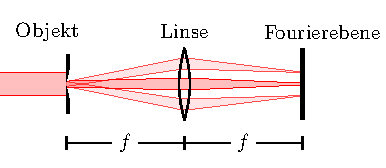
\includegraphics[scale=1]{graphs/theorie/ft-an-linse.pdf}
	\caption[Illustration: Fouriertransformation an einer Linse]{
		Ein kollimierter \\
		Laserstrahl von Links trifft auf ein Objekt (hier einen Spalt) und wird gestreut. Hier sind beispielhaft drei Strahlenverläufe eingezeichnet. Diese könnten als -1.,0. und 1. Intensitätsmaximum der Streuung interpretiert werden. Man erkennt, dass durch das Objekt die Intensitätsverteilung in der Fourierebene beeinflusst wird.
	} \label{fig:ft-an-linse}
\end{comment}


\begin{figure}[h]
	\centering
	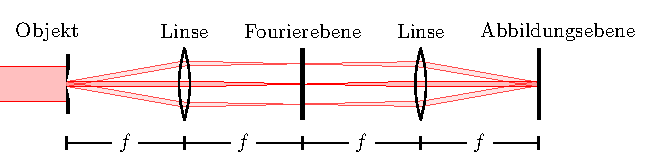
\includegraphics[scale=1]{graphs/theorie/abbildung.pdf}
	\caption[Illustration: Inverse und Fouriertransformation an Linsen]{
		Ein kollimierter Laserstrahl von links trifft auf ein Objekt (hier einen Spalt) und wird gestreut. Hier sind beispielhaft drei Strahlenverläufe eingezeichnet. Diese könnten als 1.,0. und -1. Intensitätsmaximum der Streuung interpretiert werden. Man erkennt, dass durch das Objekt die Intensitätsverteilung in der Fourierebene beeinflusst wird. Eine zweite Linse transformiert diese wieder zurück und erzeugt so eine Abbildung des Objektes.
	} \label{fig:ft-an-linse}
\end{figure}

Eine mathematische Herleitung dieser, hier nur anschaulich erläuterten Effekte, ist beispielsweise im Begleitheft zu diesem Versuch oder in\cite{universitat_gottingen_lp_????} zu finden.


Eine weitere Linse transformiert das Bild zurück und man erhält eine Abbildung des Objektes. Dies wird 